\documentclass[../../main]{subfiles}
\graphicspath{{\subfix{../../Images/}}}

\begin{document}

% TODO: Przed napisaniem tej części zastanawiałem się, jak podzielić miedzy sobą pojęcia
%architektury, struktury i pojęcia z języka angielskiego - desing. Dlaczego? No bo conajmniej pierwsze
%dwa pojęcia będą często używane w tej prace, i ja się obawiałem, że będę wykorzystywał je w własny,
%niezdefiniowany sposób (bo nie znalazłem tak naprawdę dokładnej definicji, są tylko dyfinicje dla
%poszczególnych branży, w których te pojęcia są używane).
%Po przemyśleniu zdefiniowałem ję w następujący sposób:
%Struktura - łączenie czegokolwiek posiadającego własciwości lub funkcjanolności jednego typu z
%czymkolwiek posiadającym właściwości lub funkcjanolności takiego samego typu w określony
%sposób dla stworzenia czegokolwiek z innymi właściwościami lub funkcjanolnościami.
%Architektura - łączenie czegokolwiek posiadającego własciwości lub funkcjanolności jednego typu
%z czymkolwiek posiadającym właściwości lub funkcjanolnościinnego typu w określony sposób dla
%stworzenia czegokolwiek z innymi właściwościami lub funkcjanolnościami.
%Design - struktura lub architektura stowrzona dla osiągniecia pewnego celu (IMHO najbliższe %tłumaczenie na język Polski - projekt, chociaż w języku angielskim project =/= design).
%Zostawiam to tu, aby nie zgubić. W pracę będę korzystał z tych pojęć zgodnie z tymi definicjami.}

Ten rozdział przedstawia i opisuje architektury oprogramowania w systemach wbudowanych opartych na jednostkach obliczeniowych skonstruowanych na podstawie architektury \gls{arm}'owej. Używana w tej pracy definicja pojęcia "system wbudowany" znajduje się w \hyperref[sec:zalacznik-1]{załączniku nr 1}. Omówione zostaną także cechy przedstawionych architektur oraz właściwości, które je powodują. Następnie zostaną przedstawione przykładowe realizacje tych architektur. Należy również wspomnieć, że \gls{arm} wprowadza także technologię TrustZone, która oferuje kilka dodatkowych architektur. Ponieważ celem tej technologii jest bezpieczeństwo — architektury, które ona wprowadza, nie zostaną tu omówione.

W dalszej części pracy omówiony zostanie termin "wirtualizacja" i terminy pochodne (parawirtualizacja, wirtualizacja natywna), których wyjaśnienie można znaleźć w  \hyperref[sec:zalacznik-2]{załączniku nr 2}. W załączniku tym omówione są także pojęcia separacji, translacji pamięci i przekierowywania przerwań.

Pojęcia przełączenia stanów i przełączenia kontekstu zostały wyjaśnione w \hyperref[sec:zalacznik-3]{załączniku nr 3}.

\subsection{Architektura nagi metal}

Najprostsza pod względem liczby poziomów abstrakcji architektura, składająca się ze sprzętu i aplikacji wykorzystującej ten sprzęt (\cref{fig:bare-metal}). Aby funkcjonować jako system wbudowany, potrzebna jest jednostka obliczeniowa dla wykonywania poleceń, pamięć do przechowywania poleceń, moduły wejścia/wyjścia dla kontaktu ze środowiskiem zewnętrznym i kontroler przerwań dla poinformowania aplikacji o zdarzeniach z zewnątrz. Zasoby sprzętowe są przydzielane statycznie podczas kompilacji, nie ma separacji środowisk lub uprzywilejowanego dostępu.

\begin{figure}[ht]
    \centering
    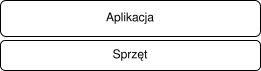
\includegraphics[width=0.55\textwidth]{Images/bare-metal.png}
    \caption{Architektura nagi metal}
    \label{fig:bare-metal}
\end{figure}

Poniżej przedstawiono najważniejsze cechy:
\begin{itemize}
    \item Prostota: architektura nie posiada poziomów abstrakcji, aplikacja kontaktuje się bezpośrednio ze sprzętem, nie ma skomplikowanych modułów do zarządzania bezpieczeństwem, np.
    \gls{mmu} lub \gls{gic};
    \item Wydajność: architektura nie posiada rozbudowanego kodu systemu operacyjnego ani    hiperwizora, nie ma translacji pamięci i przekierowania przerwań, nie ma przełączania kontekstu;
    \item Determinizm: brak konkurencji za zasoby jednostki obliczeniowej przez aplikacje, z powodu możliwej obecności tylko jednej aplikacji, pełna gwarancja reakcji na zdarzenie;
\end{itemize}

Uwzględniając powyższe cechy i właściwości, można wysnuć wniosek, że taka architektura jest przeznaczona dla małych jednostek w systemie, np. czujników, każda z których ma zdefiniowany jedyny cel. Przykładem realizacji danej architektury może być dowolna aplikacja niewykorzystująca systemu operacyjnego ani hiperwizora działająca na dowolnej architekturze \gls{arm}'owej. Chociaż najczęściej wybierana będzie jedna z architektur z rodziny \gls{m}, ponieważ są one najlepiej do tego przystosowane. Dana architektura nie stanowi przedmiotu zainteresowania w ramach tej pracy, ponieważ nie posiada oprogramowania zarządzającego dostępem do zasobów jednostki obliczeniowej.

Architektura posiadająca jedną warstwę abstrakcji, system operacyjny (\cref{fig:no-virt}) - jest to oprogramowanie systemowe, które w pełni lub częściowo (zależy od architektury systemu operacyjnego) zachowuje kontrolę nad sprzętem. Opiera się na dodatkowych modułach sprzętowych zarządzających pamięcią, którymi są najczęściej \gls{mpu}, lub też \gls{mmu}, aby oddzielić kod systemu operacyjnego od kodu aplikacji, oraz na bardziej złożonym kontrolerze przerwań, obsługującym nie tylko zdarzenia zewnętrzne, ale także zdarzenia wewnętrzne, pozwalające na zmianę stanu systemu.

\subsection{Architektura z systemem operacyjnym}

Jednostka obliczeniowa ma wbudowany podział stanów systemu: tryb aplikacji, w którym wykonywany kod nie ma dostępu do zasobów systemowych, oraz tryb systemu operacyjnego, mający dostęp do wszystkich zasobów. Dla większości systemów operacyjnych obecność funkcjonalności podziału na tryby ze strony sprzętowej, tj. obecność odpowiednich rejestrów oraz instrukcji \gls{isa}, jest obowiązkowa.

\begin{figure}[ht]
    \centering
    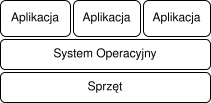
\includegraphics[width=0.55\textwidth]{Images/no-virt.png}
    \caption{Architektura z systemem operacyjnym}
    \label{fig:no-virt}
\end{figure}

Poniżej przedstawiono najważniejsze cechy:
\begin{itemize}
    \item Wysoki poziom skomplikowania: W zależności od architektury systemu operacyjnego (monolityczne jądro, mikrojądro, nanojądro), system operacyjny może posiadać różną liczbę narzędzi i funkcjonalności. Ogólnie jednak jest to bardziej złożona architektura ze względu na konieczność wykorzystania dodatkowego sprzętu systemowego oraz wprowadzenie kilku poziomów abstrakcji (np. w sterownikach).
    \item Niższa wydajność: Obecność abstrakcji w systemie operacyjnym (sterowniki,     interpretatorzy aplikacji), przełączanie stanów pomiędzy systemem operacyjnym a aplikacją, oraz przełączenie kontekstu pomiędzy aplikacjami skutkuje zmniejszeniem zasobów dostępnych dla aplikacji.
    \item Większe bezpieczeństwo: Możliwość "narzucania" zasad (definiowanie dostępów i innych ograniczeń) dla aplikacji z poziomu systemu operacyjnego oraz separacja aplikacji zwiększa bezpieczeństwo.
    \item Skalowalność: Obecność oprogramowania zarządzającego zasobami jednostki obliczeniowej pozwala na uruchomienie wielu aplikacji oraz definiowanie priorytetów dla każdej z nich oddzielnie, co umożliwia realizację wielu celów przez jeden system wbudowany.
    \item Mniejszy determinizm: W przypadku obecności wielu aplikacji pojawia się prawdopodobieństwo, że zadania przypisane każdej z tych aplikacji zostaną wykonane w innym czasie, niż przewidziano. Wynika to z konkurencji o dostęp do jednostki obliczeniowej między aplikacjami.
\end{itemize}

Taką architekturę oprogramowania można znaleźć na wszystkich architekturach \gls{arm}'owych,  t.j.: \gls{m}, \gls{a} i \gls{r}. Przykłady jej zastosowania obejmują:

\begin{itemize}
    \item FreeRTOS;
    \item Zephyr RTOS;
    \item Linux;
    \item FreeBSD, NetBSD;
    \item Windows;
    \item seL4.
\end{itemize}

Architektura z system operacyjnym będzie poruszona w tej pracy, ponieważ zawiera ona oprogramowanie zarządzające zasobami jednostki obliczeniowej, zwane także nadzorcą. Nadzorca jest częścią jądra systemu operacyjnego.

\subsection{Architektura z wirtualizacją}

Architektura z wirtualizacją jest realizowana poprzez dodania kolejnego poziomu abstrakcji do wcześniej omówionych architektur (\cref{fig:virt}). Hiperwizor może uruchamiać \gls{vm} z aplikacją w architekturze "nagi metał" jak również z systemem operacyjnym, który będzie odpowiedzialny za uruchomianie aplikacji.

\begin{figure}[h]
    \centering
    \includegraphics[width=0.65\textwidth]{Images/virt.png}
    \caption{Architektura z wirtualizacją}
    \label{fig:virt}
\end{figure}

Typowo hiperwisory wymagają odpowiedniego sprzętu dla działania (ang. virtualization support). Głównie chodzi o rozszerzenia do obsługi przerwań oraz separacji pamięci, oraz dodaniu  oddzielnego stanu jednostki obliczeniowej), np. \gls{el} w architekturach \gls{a}. W takim przypadku wirtualizacja nazywana jest natywną (ang. native virtualization, także ang. full virtualization, lub ang. hardware-accelerated virtualization).

Istnieje także możliwość stworzenia hiperwizora niezależnego od sprzętu, czyli takiego który nie wymaga odpowiedniego sprzętu do działania, jest to tzw. parawirtualizacja (ang. paravirtualization).

Poniżej przedstawiono najważniejsze cechy:
\begin{itemize}
    \item Bardzo wysoki poziom skomplikowania: Oprócz faktu, że hiperwizor jest przeznaczony do uruchamiania różnych architektur w środowisku wirtualnym, co w przypadku parawirtualizacji może być dużym wezwaniem, dochodzą również kwestie związane z komunikacją pomiędzy środowiskami oraz podziałem dostępu do sprzętu pomiędzy poszczególnymi środowiskami, w tym podziału przerwań. Dodatkowo może być wykorzystywana emulacja.
    \item Jeszcze mniejsza wydajność: Dalsze obniżenie wydajności wynika głównie z konieczności translacji pamięci, przechwytywania i wirtualizacji przerwań oraz dodatkowego przełączania stanów i kontekstu.
    \item Jeszcze większe bezpieczeństwo: Do separacji oprogramowania w pamięci dochodzi precyzyjne przypisywanie zasobów sprzętowych do poszczególnych środowisk wirtualnych.
    \item Konfigurowalny determinizm: Oznacza to, że na jednym urządzeniu można uruchomić dwie lub więcej zupełnie różnych architektur, np. "nagi metal" i system operacyjny, które charakteryzują się różnymi właściwościami deterministycznymi i rozłożyć priorytety. Można również zmienić sposób zarządzania zasobami jednostki obliczeniowej, przechodząc od dynamicznego zarządzanie do statycznego zarządzania.
\end{itemize}

Omawianą architekturę oprogramowania systemowego można spotkać na architekturach sprzętowych z rodzin \gls{a} i \gls{r}, które są wyposażone w specjalny sprzęt wspierający wirtualizację. Możliwe jest również jej uruchomienie na architekturach niewyposażonych w takie wsparcie, jednak w takim przypadku konieczne będzie zastosowanie parawirtualizacji.

Przykłady realizacji:
\begin{itemize}
    \item Jailhouse;
    \item Xen;
    \item Bao;
    \item seL4 CAmkES;
    \item KVM;
    \item Crosscon Hypervisor.
\end{itemize}

Główną uwagą w tym przypadku jest fakt, że hiperwizor jest dodatkową warstwę zarządzającą zasobami jednostki obliczeniowej, co oznacza, że jest on także punktem zainteresowania w ramach tej pracy. W przypadku, gdy w środowisku wirtualnym realizowana jest architektura z systemem operacyjnym, można mówić o zagnieżdżonym (dwupoziomowym) zarządzaniu dostępem do zasobów jednostki obliczeniowej.

\subsection{Architektura z wirtualizacją zagnieżdżoną}

Wirtualizacja zagnieżdżona (ang. nested virtualization) polega na stworzeniu \gls{vm} wewnątrz \gls{vm} (\cref{fig:virt-nested}), co wiąże się z dodaniem też dodanie dodatkowego hiperwizora, który może być nazywany "hiperwizorem podrzędnym".

\begin{figure}[h]
    \centering
    \includegraphics[width=\textwidth]{Images/virt-nested.png}
    \caption{Architektura z wirtualizacją zagnieżdżona}
    \label{fig:virt-nested}
\end{figure}

Aktualnie architektury \gls{arm}'owe wspierają tę architekturę częściowo, tzn. nie ma ani dodanego kolejnego \gls{el}, ani wsparcia dla trzypoziomowej translacji pamięci, ani dedykowanych  mechanizmów przekierowywania przerwań, jest jedynie podstawowe wsparcie w postaci rozszerzeń do niektórych rejestrów w architekturach z rodziny \gls{a} \cite{nestvirtarm}.

Ta architektura dodaje kolejną warstwę z oprogramowaniem, które zarządza dostępem do zasobów jednostki obliczeniowej. Oprogramowanie to znajduje się w hiperwizorze podrzędnym, co, w przypadku gdy w VM utworzonej przez hiperwizor podrzędny jest wykorzystywana architektura z systemem operacyjnym, skutkuje trzema poziomami zarządzania dostępem do jednostki obliczeniowej: oprogramowanie w hiperwizorze nadrzędnym, oprogramowanie w hiperwizorze podrzędnym i oprogramowanie w systemie operacyjnym. To stanowiłoby interesujący punkt dla badań, gdyby nie słabe wsparcie tej architektury w społeczeństwie systemów wbudowanych, co powoduje liczne problemy, które nie stanowią centrum uwagi tej pracy \cite{nestvirtarm}. Dlatego ta architektura nie będzie omawiana w ramach tej pracy.

\end{document}